% LTeX: language=spanish

\chapter{Introducción}

Con la transición a la computación en la nube, surgen los \textbf{centros de procesamiento de datos} como sistemas de procesamiento principales. Atrás se han quedado los tiempos de los ordenadores personales como principal fuente de trabajo. El auge de estos centros ha creado una carrera por optimizar la capacidad de cómputo por unidad de espacio. 

Sin embargo, cualquier dispositivo tecnológico está condenado a producir calor para operar. Esto es inevitable. Teniendo en cuenta la concentración de equipamiento que se produce en un centro de datos, disipar el calor producido se vuelve un problema serio. Si no se refrigeraran, la vida útil de sus componentes se acortaría, su capacidad de cómputo se vería mermada, lo cual haría que aumentara el \textit{downtime} significativamente. Una mala gestión produce efectos negativos en cadena. Además, las consecuencias medioambientales serían desastrosas. Por todo estos motivos, debemos buscar métodos de transferencia de calor. 

La solución a nuestros problemas energéticos la aportarán los \textbf{sistemas de refrigeración}. Estos sistemas conseguirán una reducción de la temperatura en el centro de datos; tanto para componente individual como para el edificio en su conjunto. No obstante, su funcionamiento no es trivial: debemos analizar cómo de eficaces son, así como su eficiencia. Un sistema de refrigeración poco eficaz no disminuirá la temperatura de los componentes lo suficiente, pero tampoco podemos permitirnos malgastar electricidad. 

En este trabajo abordaremos estos dos conceptos: sistemas de refrigeración y su consumo. Estudiaremos las diferentes técnicas que se emplean en un centro de datos, comparando las diferentes soluciones.

Específicamente, vamos a analizar cómo se comportan las diferentes técnicas de refrigeración por aire [\ref{aire}], agua [\ref{awa}] e inmersión [\ref{inmersion}]; comprobaremos algunas de las soluciones que han propuesto diferentes empresas [\ref{empresas}] y exploraremos el futuro de la industria [\ref{futuro}].




\chapter{Preliminares}

Los \textbf{centros de procesamiento de datos} (CPD; en inglés, \textit{data centers}) son los lugares físicos donde se instalan sistemas de cómputo y sus componentes asociados \cite{wikipedia-datacenter}. El fin de estos sistemas es muy diverso: pueden usarse para almacenar información, alojar una página web, o proveer un servicio de procesamiento para empresas. Algunos de los componentes que forman un CPD son routers, switches, firewalls o sistemas de almacenamiento masivo de datos. 

Para que funcionen a pleno rendimiento, es esencial saber cómo organizar estos sistemas; tanto informática como físicamente. No solo es imprescindible gestionar servidores, sino que debemos adaptar el espacio físico disponible a nuestra maquinaria. Generalmente, no dispondremos de mucho; y sumado a una alta densidad de dispositivos funcionando a pleno rendimiento, llega el inevitable archienemigo de la electricidad: \textbf{el calor}.

\section{Los sistema de refrigeración}

La solución a nuestros problemas de temperatura la aportarán los \textbf{sistemas de refrigeración}, también conocidos como sistemas de climatización. Todas las técnicas de refrigeración tienen como objetivo principal \textbf{reducir la temperatura de un equipo}, aunque lo consigan de diferente manera. Debido al poco espacio disponible en un sistema, un sistema de refrigeración usará algún medio para transferir el calor a otro lugar. Esta es una forma muy eficiente de refrigerar un sistema, pues resulta más sencillo mover todo el calor a otra parte para tratarlo en un lugar específico, en lugar de trabajar equipo a equipo. Esta es la misma base que se utiliza en los ordenadores personales, aunque a una escala mucho mayor.

En esencia, un sistema de climatización suele estar formado por los siguientes componentes:

\begin{itemize}
    \item \textbf{Un generador del medio a utilizar para transferir el calor}.
    \item \textbf{Una vía por la que viaja el medio}. Pueden ser cables, el aire, un pasillo...
    \item \textbf{Una fase de transferencia de calor} del sistema o habitación al medio.
    \item \textbf{Una forma de enfriar} el medio.
\end{itemize}

Además, existen tres vías principales de transferencia de calor:

\begin{itemize}
    \item \textbf{A través del aire}: se basan en conductos de aire para enfriar los diferentes dispositivos. Estos conductos bombean aire frío hacia los equipamientos y luego recogen el aire caliente que sale de estos. De esta forma, se consigue separar el aire caliente del frío. Un importante inconveniente es que este tipo de sistemas requiere un gran consumo de energía.
    \item \textbf{A través del agua}: utilizan grandes contenedores de agua fría con el fin de bombear el agua a través de tuberías que pasan entre los dispositivos y los racks. Es importante mantener siempre una barrera entre los dispositivos y el agua que circula, pues si se produce contacto entre ellos se podrían dañar los componentes (conocido como fugas o \textit{leaks}).
    \item \textbf{Inmersión}: con esta técnica, los equipos de IT se sumergen en un fluido dieléctrico que no conduce la electricidad, pero que sí es capaz de mover el calor fuera de los microprocesadores. Este tipo de sistemas destaca por ser el más eficiente sin necesidad de necesitar sistemas de refrigeración con gases fluorados.
\end{itemize}

La escala del sistema de refrigeración dependerá de cómo de ambicioso sea el centro de datos. Teniendo en cuenta la \textit{tier} del CPD \cite{cofrico}, se usará un tipo u otro; dependiendo de la robustez que aporten.

\section{Eficiencia energética de los sistemas de refrigeración}

El sistema de refrigeración puede suponer hasta un 40\% del consumo energético del CPD. Una parte importante de este 40\% la componen los ventiladores (12\% del total) y los enfriadores del agua (14\% del total), de acuerdo a los datos de \cite{ZHANG2021102253}. Para facilitar la visualización de estos datos puede verse \eqref{consumo_energetico}.

\begin{figure}
    \begin{center}
        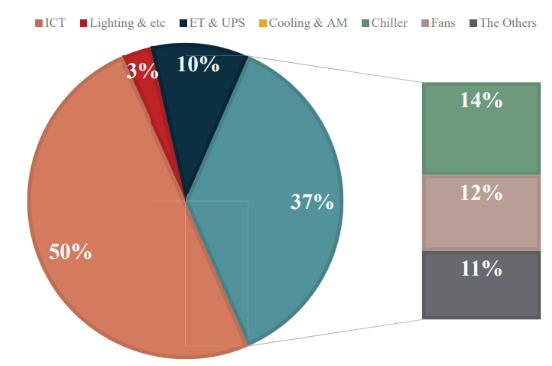
\includegraphics[scale=1]{consumo}
        \caption{Consumo energético del CPD.}
        \label{consumo_energetico}
    \end{center}
\end{figure}

Se estima que, en 2020, el consumo de los centros de datos supuso un 1 - 1.5\% de la producción de electricidad global \cite{mytton-dc}. Con la llegada de la pandemia y la transición al trabajo remoto, esta cifra ha aumentado en los últimos dos años; y la tendencia es que continúe en crecimiento. Aunque las arquitecturas modernas necesitan menos energía para operar con un uso bajo, el consumo medio de un rack es de 7 kW, llegando a picos de incluso 20 kW por rack \cite{datacenters-density}. Por lo tanto, será esencial mantener bajo control el consumo energético del CPD. 

\section{Green IT}

El consumo de un centro de procesamiento de datos proviene principalmente de su climatización y el equipamiento del mismo.

Con el objetivo de reducir el impacto climático de los centros de procesamiento de datos y disminuir los costes de consumo de los mismos, el Green IT propone diversas estrategias \cite{techtargetgreen}, entre las que se encuentran materiales de construcción de bajo impacto medioambiental, reciclar residuos tecnológicos, uso de energías renovables, consolidación de servidores o virtualización.

El uso correcto de las Green IT proporciona diversas ventajas, entre las que se encuentran la reducción de costes a largo plazo; un menor requerimiento de espacio; así como la reducción de las emisiones de carbono, generación aguas residuales, y consumo de agua y electricidad.

Algunas de las acciones que se pueden llevar a cabo para reducir los residuos electrónicos desde los centros de procesamiento de datos se muestran en \eqref{waste}.

\begin{figure}
    \begin{center}
        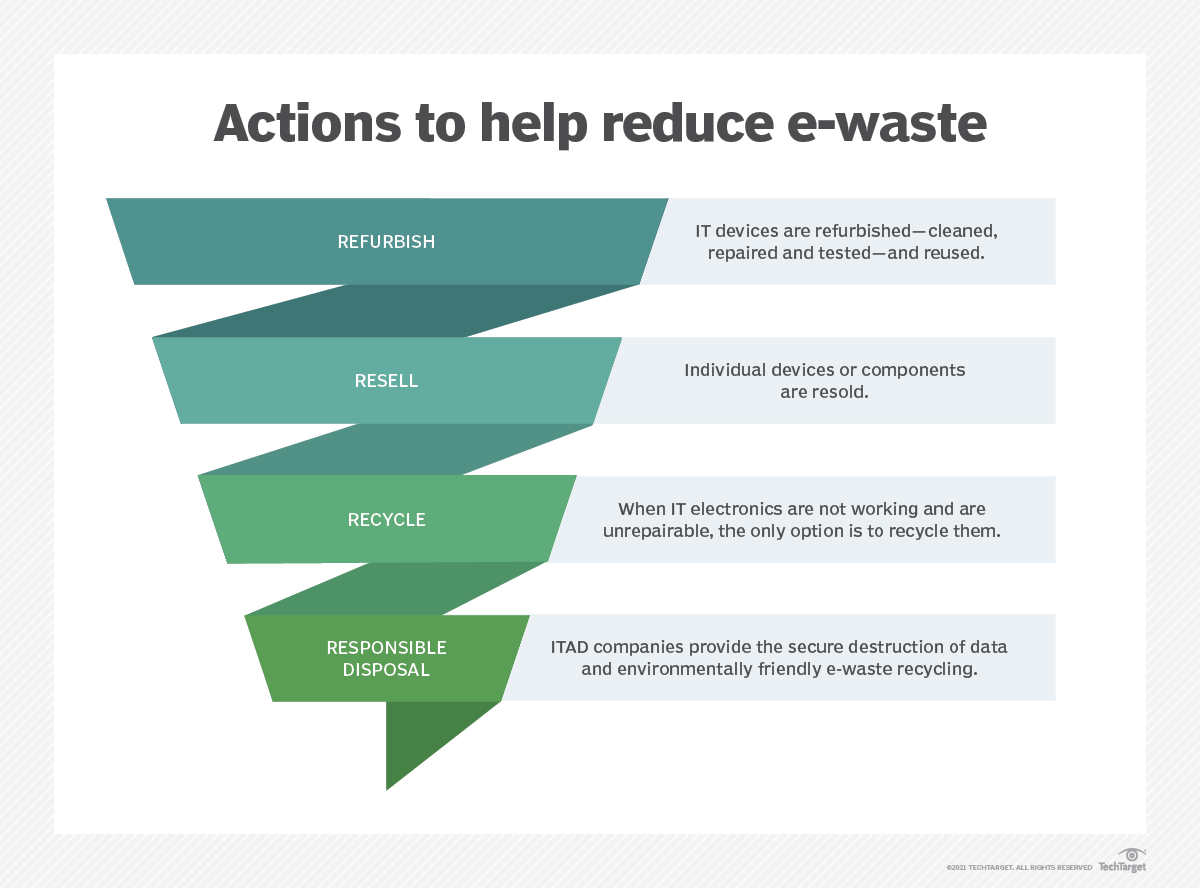
\includegraphics[scale=0.3]{actions_to_help_reduce_ewaste}
        \caption{Acciones para ayudar a reducir los residuos tecnológicos \cite{techtargetgreen}.}
        \label{waste}
    \end{center}
\end{figure}

Durante los últimos años se ha hecho especial énfasis en la implantación y puesta en práctica de las Green IT, lo que ha propiciado a que surjan empresas específicas para este propósito. Un ejemplo de estas es Equinix \cite{equinix}, quierens ayudan a diseñar los centros de procesamiento de datos para que sean medioambientalmente sostenibles. Para ello, proponen diversas soluciones como el aislamiento térmico o sistemas de iluminación de bajo consumo.

Actualmente España se encuentra a la cabeza de las invenciones de tecnología verde en Europa, ocupando el sexto lugar. Esto se debe principalmente a la preocupación que se ha extendido en Europa por el cambio climático, lanzando así diversos proyectos para tratar de frenarlo. Esta información puede ampliarse en \cite{efe}.



\chapter{Desarrollo}

En este capítulo vamos a comentar los distintos tipos de técnicas de refrigeración que hay: aire, agua e inmersión. De cada tipo estudiaremos y desarrollaremos las distintas técnicas que existen, junto a esquemas gráficos que faciliten su comprensión.

\section{Técnicas de refrigeración}

\subsection{Aire} \label{aire}

En este apartado estudiaremos las distintas técnicas cuya vía principal para climatizar los CPD es el aire.

\subsubsection{Free cooling}

Free cooling \cite{gento} es una técnica efectiva para asegurar que el flujo de temperatura de un centro de procesamiento de datos está funcionando adecuadamente. Esta técnica requiere de un coste mínimo, por lo que reduce los gastos totales de la refrigeración del CPD.

Este método se basa en la economización de aire. Para ello se usa el aire del exterior del centro de procesamiento de datos para regular la temperatura de los equipos del interior del CPD, dejándolo entrar a este.

Generalmente, con el fin de evitar que entre humedad o partículas contaminantes se suele realizar un filtrado del aire.

En la imagen \eqref{free_coling} podemos observar un esquema del funcionamiento de esta técnica.

\begin{figure}
    \begin{center}
        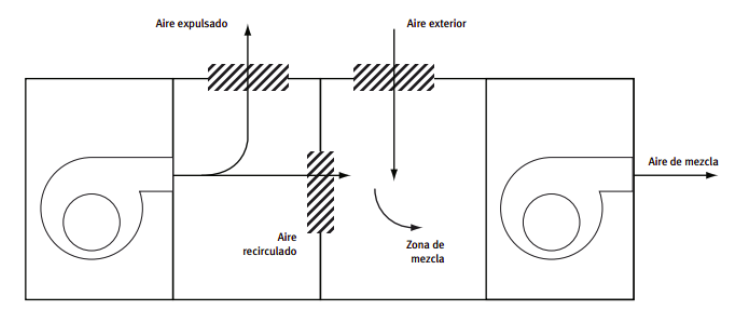
\includegraphics[scale=1]{free_cooling}
        \caption{Esquema del free cooling.}
        \label{free_coling}
    \end{center}
\end{figure}

Esta técnica tiene varias ventajas, pues permite ahorrar y mejora la calidad del aire interior. Sin embargo, requiere de un mínimo consumo y de un mecanismo complejo de ventiladores, compuertas y filtros.

\subsubsection{Pasillos calientes y fríos}

Esta técnica tiene como objetivo separar por completo el aire frío proveniente del aire acondicionado y el aire caliente que expulsan los equipos. Para ello, se aprovecha el diseño de los racks de servidores y la disposición de los mismos en el centro de procesamiento de datos. Esto es, se alinean los racks en filas alternas (frío/caliente), dejando todas las entradas de aire frío hacia un lado y las salidas de aire caliente hacia el otro. Así, las filas compuestas por frentes de racks se llaman pasillos fríos, que suelen enfrentar a los conductos de salida del aire acondicionado, y la parte trasera de los racks, por donde se expulsa el aire caliente, se denominan pasillos calientes, que suelen conectarse a los conductos de retorno del aire acondicionado.

En las imágenes \eqref{pasillos} y \eqref{traditional_cooling} podemos observar unos esquemas del funcionamiento de esta técnica.

\begin{figure}
    \begin{center}
        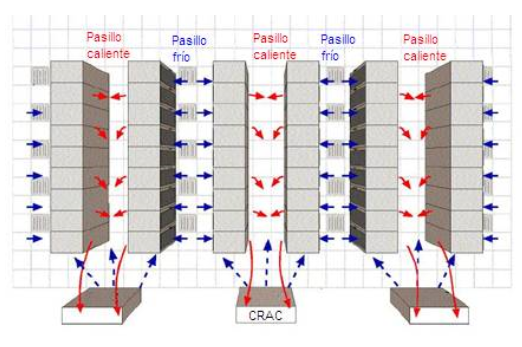
\includegraphics[scale=0.7]{pasillos}
        \caption{Esquema de los pasillos calientes y fríos. Fuente: \cite{Kelvion}.}
        \label{pasillos}
    \end{center}
\end{figure}

Esta técnica suele combinarse con el método de falsos suelos y techos para facilitar el paso del aire.

Además, mediante esta técnica se conserva la energía y se reducen los costes de enfriamiento por la gestión del flujo de aire.

\begin{figure}
    \begin{center}
        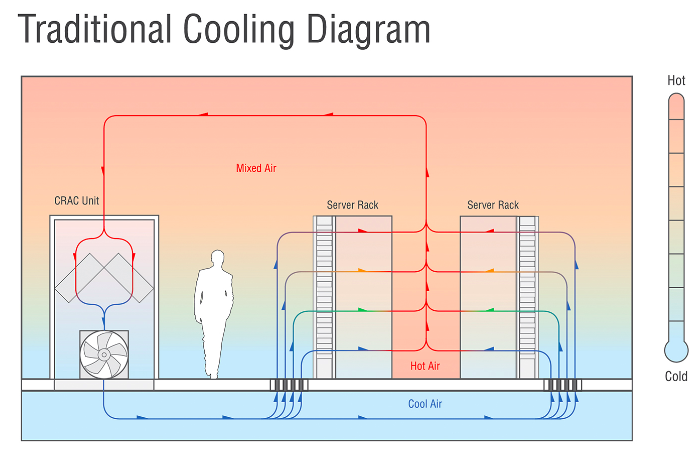
\includegraphics[scale=1]{traditional_cooling_diagram}
        \caption{Diagrama de enfriamiento tradicional.}
        \label{traditional_cooling}
    \end{center}
\end{figure}

\subsubsection{Confinamiento de zonas}

Esta técnica se basa en aislar los pasillos fríos de los calientes mediante la colocación de cerramientos. De esta forma, los pasillos podrán recibir la circulación de los flujos de aire correspondiente sin que se produzca una mezcla de corrientes sin control.

En la imagen \eqref{hot_aisle} podemos observar un esquema del funcionamiento de esta técnica.

\begin{figure}
    \begin{center}
        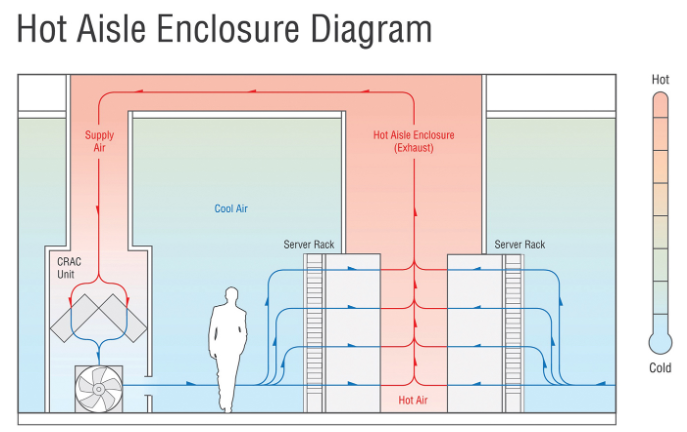
\includegraphics[scale=1]{hot_aisle}
        \caption{Diagrama de cerramiento de pasillo caliente.}
        \label{hot_aisle}
    \end{center}
\end{figure}

\subsubsection{Refrigeración adiabática}

Esta técnica es capaz de utilizar la baja humedad relativa del aire para incorporar agua y evaporarla, por lo que consigue lograr una importante reducción de temperatura. Una ventaja es que no necesita un importante consumo energético.

En la imagen \eqref{adiabatic_coolers} se muestra un dispositivo para realizar el enfriamiento adiabático.

\begin{figure}
    \begin{center}
        % TODO: añadir referencia de kfocus
        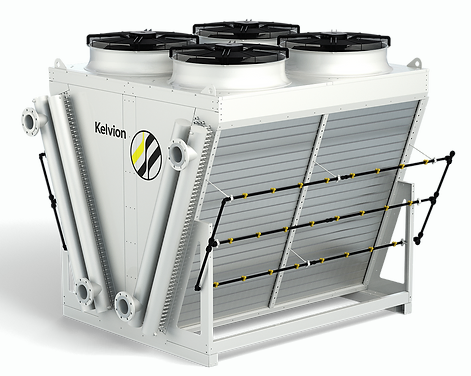
\includegraphics[scale=1]{adiabatic_coolers}
        \caption{Enfriamientos adiabáticos}
        \label{adiabatic_coolers}
    \end{center}
\end{figure}

\subsubsection{In-Rack Heat Extraction}

La idea de este método de refrigeración se basa en extraer el calor que se genera dentro del rack para que ni siquiera entre en la sala de servidores.

\subsubsection{Aire acondicionado para la sala de ordenadores (CRAC)}

Las unidades CRAC son similares a equipos usuales de aire acondicionado que funcionan gracias a un compresor, el cual atrae aire a través de una unidad cargada con refrigerante. De esta manera, se introduce el aire frío en el centro de procesamiento de datos.

Son bastante comunes en muchos centros de datos, ya que a pesar de su alto consumo de energía, el coste del equipo es muy bajo.

En estas unidades se suelen usar aparatos como \eqref{custom_air_coils}.

\subsubsection{Controlador de aire para la sala de ordenadores (CRAH)}

Una unidad CRAH funciona dentro de un sistema más amplio que involucra una planta de agua enfriada. Este agua fluye a través de un conducto de enfriamiento dentro de la unidad, que luego usa ventiladores de modulación para extraer aire del exterior de la instalación. Estas unidades serán más eficientes si se usan en lugares con temperaturas más frías, pues tendrán que enfriar menos el aire exterior.

En estas unidades se suelen usar aparatos como \eqref{custom_air_coils}.

\subsubsection{Refrigeración vectorial calibrada (CVC)}

Esta tecnología de enfriamiento está hecha específicamente para servidores de alta densidad. Optimiza la ruta del flujo de aire a través del equipo para permitir que el sistema de enfriamiento maneje el calor de manera más efectiva, lo que hace posible aumentar la proporción de placas de circuito por chasis de servidor y utilizar menos \textit{enthusiasts}.

\subsubsection{Falsos suelos y techos}

Los suelos y techos técnicos para centros de datos son suelos y techos que pueden instalarse a distintas alturas, dejando un hueco entre esta instalación y los suelos y techos "reales".

Es usual que los suelos consistan en rejillas de ventilación, pues son convenientes para servicios de refrigeración, eléctricos y mecánicos. De esta forma, con menos gasto de energía se puede ayudar en la refrigeración de los servidores, por ejemplo centrando las salidas de aire bajo las máquinas.

También resulta útil para facilitar el acceso al cableado. En este aspecto, el falso techo supone más problemas que el suelo, pues requiere usar guías y escaleras para acceder a él, pero con el falso suelo solo hay que levantar las baldosas y realizar los ajustes necesarios.

Por último, cabe destacar que estos suelos dan flexibilidad, pues pueden instalarse a la altura que se requiera y pueden reutilizarse si se reformara el CPD o se cambiara la localización del mismo.

\subsubsection{Expansión directa (DX cooling)}

Esta técnica utiliza los principios de la termodinámica para transferir calor de un área a otra a través de la evaporación y condensación de un refrigerante, que sirve como medio a través del cual el calor se captura y se elimina de un área y se libera en otra. Por ejemplo, los aires acondicionados usan este mecanismo para mover el calor de una habitación hacia el exterior.

Este sistema tiene las siguientes componentes:

\begin{itemize}
    \item {\textbf{El refrigerante}}, que es el medio que fluye a través del sistema, recolectando y disipando el calor en diferentes áreas.
    \item \textbf{El compresor}, que es una carga de motor eléctrico y suministra la energía para impulsar el refrigerante a través del sistema.
    \item \textbf{El evaporador}, que recoge el calor del recinto y facilita la ebullición del refrigerante.
    \item \textbf{El condensador}, que disipa el calor en el medio ambiente al permitir que el refrigerante vuelva a su estado líquido.
    \item \textbf{La válvula de expansión}, que actúa como regulador entre el lado de alta y baja presión del sistema y permite la caída de presión y temperatura necesaria para facilitar la expansión directa.
\end{itemize}

\subsection{Agua} \label{awa}

En este apartado estudiaremos las distintas técnicas cuya vía principal para climatizar los CDP es el agua.

\subsubsection{Sistema de agua helada}

Este método se usa comúnmente en centros de datos de tamaño mediano a grande que usan agua caliente para enfriar el aire que producen los controladores de aire (CRAH). Para ello, se usa una planta enfriadora para suministrar el agua.

\subsubsection{Enfriamiento evaporativo}

Esta técnica expone el aire caliente al agua, lo que produce la evaporación del agua y así extraer el calor del aire. Este sistema es extremadamente eficiente desde el punto de vista energético, sin embargo utilizará mucha agua.

\subsection{Inmersión} \label{inmersion}

En este apartado estudiaremos las distintas técnicas cuya vía principal para climatizar los CDP es la inmersión. Existen máquinas muy útiles para este tipo de técnica, como por ejemplo la de la figura \eqref{air_cooled_condensers}.

\subsubsection{Refrigeración por inmersión}

En este método, el hardware se sumerge en un fluido dieléctrico no conductor y no inflamable, introduciendo tanto el líquido como el hardware en un contenedor a prueba de fugas. De esta manera, el líquido absorbe el calor mientras que el agua caliente se convierte en vapor, para luego condensarse al enfriarse y vuelve al líquido refrigerante, ayudando así a que este se enfríe de nuevo.

Cabe destacar que esta técnica es muy eficaz, pues el fluido absorbe el calor mucho más eficientemente que el aire.

\section{Soluciones corporativas} \label{empresas}

En esta sección presentaremos algunas empresas que se dedican a suministrar los productos necesarios para conseguir soluciones de refrigeración para centros de datos.

Un ejemplo es la empresa Systemair \cite{systemair}, que ofrece una gran variedad de productos en este catálogo para asegurar sistemas de refrigeración energéticamente eficientes, tales como unidades de enfriamiento gratuito, sistemas de enfriamiento evaporativo compacto con pre enfriamiento del aire exterior, condensadores para la expansión directa, etc.

Otra alternativa es Clysema \cite{clysema}, una empresa de servicios energéticos enfocada a mejorar la eficiencia energética de las instalaciones. Ofrecen servicios de gestión y optimización, auditoría, ejecución y mantenimiento.

Otras empresas que están ayudando a innovar la industria de los centros de datos son LiquidStack \cite{liquidstack}, Submer \cite{submer}, Usystems \cite{usystems}, Munters, \cite{munters}, Green Revolution Cooling \cite{GRC}, STULZ \cite{stulz}, etc.

La empresa Kelvion \cite{Kelvion} también ofrece métodos eficientes de refrigeración y disipación del calor. En su página web podemos observar todos los dispositivos que ofrece para las distintas técnicas comentadas, como por ejemplo enfriadores secos \eqref{fig:dry_cooler_cooling_tower} (a), Storre de refrigeración \eqref{fig:dry_cooler_cooling_tower} (b), bobinas de aire personalizadas \eqref{fig:custom_air_coils_air_cooled_condensers} (a), condensadores enfriados por aire \eqref{fig:custom_air_coils_air_cooled_condensers} (b), bomba dieléctrica \eqref{dielectric_pump}, etc.

\begin{figure}%
    \centering
    \subfloat[][]{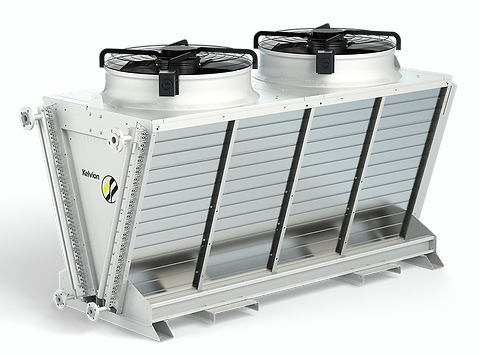
\includegraphics[scale=0.7]{dry_cooler}}%
    \qquad
    \subfloat[][]{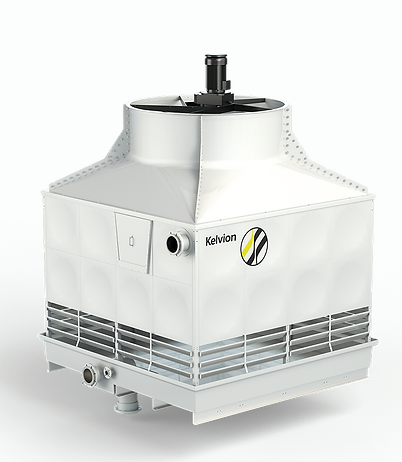
\includegraphics[scale=0.7]{cooling_tower}}
    \caption{Enfriadores secos (a) y torre de refrigeración (b). Fuente: \cite{Kelvion}}%
    \label{fig:dry_cooler_cooling_tower}%
\end{figure}

\begin{figure}%
    \centering
    \subfloat[][]{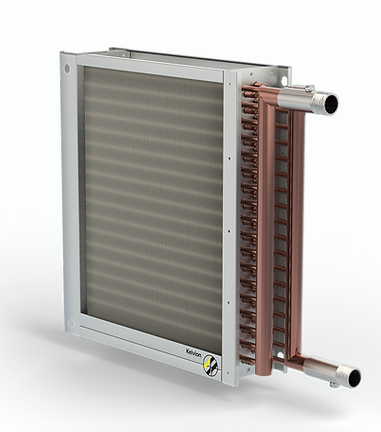
\includegraphics[scale=0.7]{custom_air_coils}}%
    \qquad
    \subfloat[][]{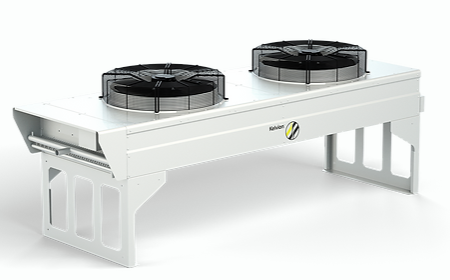
\includegraphics[scale=0.7]{air_cooled_condensers}}
    \caption{Bobina de aire personalizadas (a) y condensadores enfriados por aire (b). Fuente: \cite{Kelvion}}%
    \label{fig:custom_air_coils_air_cooled_condensers}%
\end{figure}

\begin{figure}[H]
    \begin{center}
        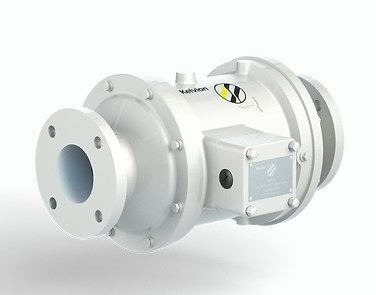
\includegraphics[scale=0.7]{dielectric_pump}
        \caption{Bomba dieléctrica. Fuente: \cite{Kelvion}.}
        \label{dielectric_pump}
    \end{center}
\end{figure}

\section{Futuro} \label{futuro}

Desde hace varios años, los centros de procesamiento de datos han incrementado su potencia y número de servidores significativamente, lo que implica la necesidad de encontrar métodos de enfriamiento más eficaces y mejores para poder enfriar estos centros de datos.

Por tanto, actualmente se están investigando nuevas técnicas de enfriamiento que se espera que puedan ponerse en práctica lo antes posible. Principalmente se está trabajando sobre técnicas con refrigeración líquida, ya que son mucho más efectivas, pues los fluidos absorben mejor el calor que el aire.

\subsection{Tecnologías de refrigeración líquida}

A diferencia del enfriamiento por aire, que requiere mucha energía e introduce contaminantes y condensación en el centro de datos, un sistema de enfriamiento líquido es más limpio, más escalable y altamente específico. Actualmente, se están desarrollando dos métodos: enfriamiento por inmersión total y enfriamiento directo del chip.

\subsubsection{Refrigeración directa del chip}

La refrigeración directa del chip usa tuberías que transportan el líquido refrigerante directamente a una placa fría que se sitúa encima de los chips de una placa base para extraer el calor. El calor extraído se lleva a un circuito de agua enfriada para ser transportado de nuevo a la planta de enfriamiento de la instalación y expulsado al exterior.

Este método proporciona una forma muy eficaz de enfriamiento para centros de datos que usan mucha potencia y, por tanto, necesitan métodos muy potentes de enfriamiento.

\chapter{Conclusiones}

En este trabajo hemos estudiado y desarrollado los sistemas de climatización, junto con los distintos tipos de técnicas de refrigeración: aire, agua e inmersión. De cada uno de estos tipos, hemos detallado las distintas técnicas de refrigeración, incluyendo esquemas gráficos para facilitar la comprensión. También hemos comentado algunas soluciones corporativas, esto es, empresas que poseen productos y maquinaria para simular algunas de las técnicas comentadas. Finalmente, hemos hablado de algunas propuestas que no están desarrolladas completamente actualmente y que serán mucho más eficientes. Por lo que podemos afirmar que los objetivos de este trabajo se han completado en su totalidad.

Para finalizar, podemos concluir que las técnicas de enfriamiento que se basan en refrigeración líquida son las más efectivas y que se deben investigar más en el futuro. Además debemos evitar las técnicas que requieran mucha energía y que introduzcan contaminantes y condensación, y desarrollar técnicas más escalables y basadas en las Green IT. Con estas recomendaciones, podremos reducir el impacto climático y disminuir los costes de consumo de los centros de procesamiento de datos.


\begin{figure}%
    \centering
    \subfloat[][]{...figure code...}%
    \qquad
    \subfloat[][]{...figure code...}
    \caption{Here are the first two figures of a continued figure.}%
    \label{fig:cont}%
\end{figure}

\begin{figure}%
    \ContinuedFloat
    \centering
    \subfloat[][]{...figure code...}%
    \qquad
    \subfloat[][]{...figure code...}
    \caption[]{Here are the last two figures of a continued figure.}%
    \label{fig:cont}%
\end{figure}